\chapter{Evaluation}
\label{ch:evaluation}
This chapter provides the experimental clustering results of word-embedding based clustering algorithm, traditional probabilistic based clustering algorithm and our model, and evaluates them by calculating the coherence. Moreover, the application of our model TTM on the COVID-19 dataset and the visualization result combined with analysis will also be displayed in this chapter.


\section{Evaluation Method}
To evaluate the performance of the unsupervised clustering model, the traditional methods for model evaluation such as cross-validation cannot work. Due to the particularity of the topic model, the obtained result can be displayed as the top words for each topic, which means the performance of the text clustering can be evaluated by human judgments, if most of the clustered topics (with the top words) have interpretable meaning, the performance of this model can be considered good. However, based on some experiments on training the models, most of the generated topics are hard to interpret, which makes evaluating the topics by human judgment difficult and because there is no unified standard for human to score the topics, it is also hard to compare the performance of different models. 

Topic coherence measures have been proposed to determine whether the topic is good or not based on the interpretability of the top words \cite{mimno2011optimizing, newman2010automatic}. Roder et al. \cite{roder2015exploring} proposed a framework allows the existing coherence measures and new measures that combined the basic components to compute the coherence, and the experiment showed the results have a positive correlation with human ratings. 

There are some python libraries provide APIs to compute the coherence, and for convenience, we adopt an online service \href{https://palmetto.demos.dice-research.org}{Palmetto}, which can return the coherence value of the word set by simply putting the top words of the topic and choose a coherence measure.

We choose $C_P$ and $C_A$ to evaluate the topics generated from our model. $C_P$ computes the coherence based on a sliding window, a one-preceding segmentation of the words and Fitelson's coherence \cite{m2020topic}. It uses a sliding window to derive the word co-occurrence counts of the word set, and for each word, uses the confirmation measures of Fitelson's coherence to calculate the confirmation to its preceding word. And the coherence result is the mean value of the confirmation measure results. While $C_A$ based on a context window, word pairs, normalized pointwise mutual information (NPMI) and the cosine similarity \cite{m2020topic}. It uses a context window to retrieve the co-occurrence counts for the word set, which is used to calculate the NPMI of each word to every other word and generate a vector for each word. Then compute the cosine similarity between all the word pairs and the coherence result is the mean value of those similarities.

\section{Experimental Result}

To evaluate and compare the models, we use the same test dataset as the input of the experiments. Since our model is expected to apply to short texts (Tweets), we tend to choose the short texts datasets as the test data. A SearchSnippets dataset, which contains 12295 documents and 5547 words from the results of web search transactions in eight different domains, is found to suit our experiments. And the number of cluster in the experiments is set to eight that same with the number of topics in the test dataset. 

Table \ref{table_1} shows the experimental result of K-means clustering algorithm. Few of the topics are interpretable, but generally the coherence score is low and there are topics obtained negative scores. It demonstrates that a more advanced model should be used to get higher coherence scores.

\begin{table}[htbp]
\centering
\begin{tabular}{|c|c|c|c|}
\hline
Topic ID & Top words & $C_A$ & $C_P$\\
\hline
1 & \tabincell{l}{research edu gov information project \\science papers journal issues topics} & 0.101 & 0.169\\
\hline
2 & \tabincell{l}{wikipedia encyclopedia wiki system article \\computer film united culture science} & 0.235 & 0.029\\
\hline
3 &\tabincell{l}{news com sports information football \\articles health net reviews statistics} & 0.093 & -0.383\\
\hline
4 & \tabincell{l}{information gov home online health \\business world web music index} & 0.146 & 0.17\\
\hline
5 & \tabincell{l}{edu university department science computer \\school theory course theoretical information} & 0.352 & 0.376\\
\hline
6 & \tabincell{l}{amazon com books music life theory \\political online computer democracy} & 0.173 & -0.123\\
\hline
7 & \tabincell{l}{com sports online definition world \\information search games index web} & 0.159 & 0.036\\
\hline
8 & \tabincell{l}{movie movies film com reviews \\american database video news guide} & 0.177 & 0.065\\
\hline
 & & 1.436 & 0.339\\
\hline
\end{tabular}
\caption{Experimental Result of K-means}
\label{table_1}
\end{table}

The following table \ref{table_2} shows the experimental result of LDA. Due to the sparsity problem which discussed in section \ref{topicmodel}, the performance of LDA is not good. 

\begin{table}[htbp]
\centering
\begin{tabular}{|c|c|c|c|}
\hline
Topic ID & Top words & $C_A$ & $C_P$\\
\hline
1 & \tabincell{l}{games game sports play espn \\scores political com schedule news} & 0.207 & 0.103\\
\hline
2 & \tabincell{l}{football club bbc wikipedia imdb \\title cup event encyclopedia diagnosis} & 0.157 & -0.008\\
\hline
3 &\tabincell{l}{party union governing diet print \\community beats elected teacher math} & 0.069 & -0.221\\
\hline
4 & \tabincell{l}{tournament sport sports yahoo news \\directory coverage online com events} & 0.218 & 0.213\\
\hline
5 & \tabincell{l}{culture calendar school civil texas \\lessons liberal master phd instruction} & 0.152 & 0.124\\
\hline
6 & \tabincell{l}{sports physical nuclear rules weapons \\wins baltimore prize institution statistics} & 0.221 & -0.408\\
\hline
7 & \tabincell{l}{republic england theoretical reform london \\san merchandise research chicago political} & 0.134 & -0.027\\
\hline
8 & \tabincell{l}{tickets australian newspaper theatre britannica \\magazine germany minister conditions physics} & 0.167 & -0.036\\
\hline
 & & 1.325 & -0.26\\
\hline
\end{tabular}
\caption{Experimental Result of LDA}
\label{table_2}
\end{table}

Table \ref{table_3} is the experimental result of BTM. The parameters $\alpha$ and $\beta$ are both set to 0.5, and the iteration is set to 500 times to ensure the Gibbs sampling converged. Combined with LDA, both $C_A$ and $C_P$ scores of BTM are distinct higher than that of LDA, and as for human judgement, there are some topics having interpretable meaning such as topic 5 is about sports, topic 6 is about computer and topic 7 related to health.

\begin{table}[htbp]
\centering
\begin{tabular}{|c|c|c|c|}
\hline
Topic ID & Top words & $C_A$ & $C_P$\\
\hline
1 & \tabincell{l}{business com amazon market theory \\news trad information wikipedia stock} & 0.183 & 0.009\\
\hline
2 & \tabincell{l}{research edu science school information \\university journal computer department home} & 0.240 & 0.350\\
\hline
3 &\tabincell{l}{music movie com film movies \\news art video online fashion} & 0.176 & -0.086\\
\hline
4 & \tabincell{l}{wikipedia political culture system encyclopedia \\wiki party government democracy information} & 0.262 & 0.249\\
\hline
5 & \tabincell{l}{news sports football com games \\soccer game world tennis match} & 0.203 & 0.252\\
\hline
6 & \tabincell{l}{computer software web internet memory \\intel programming com wikipedia device} & 0.202 & 0.233\\
\hline
7 & \tabincell{l}{health information cancer gov medical \\news disease healthy nutrition hiv} & 0.233 & 0.555\\
\hline
8 & \tabincell{l}{amazon theory physics edu theoretical \\books theorem philosophy mathematical com} & 0.270 & -0.041\\
\hline
 & & 1.593 & 1.521\\
\hline
\end{tabular}
\caption{Experimental Result of BTM}
\label{table_3}
\end{table}

The following table \ref{table_4}shows the experimental result of TTM, where the parameters $\alpha$ $\beta$ and the iteration are all same as those in the experimental of BTM. It is found that both $C_A$ and $C_P$ coherence scores are higher than the traditional BTM. In addition to the topics that are also extracted by BTM such as sports (topic 5) and health(topic 7), TTM also explored more latent topics related to political (topic 6) and finance (topic 4). Moreover, the capability to distinguish the topics with semantically similarity becomes little better. For example, topic 1 and topic 8 are both related to university, but it can tell that topic 1 focus on the school while topic 8 more talks about some programs. However, the impact of high-frequency words on the clustering results is aggravated in TTM, so that some high-frequency words such as 'software' might appears on most of the topics.

\begin{table}[htbp]
\centering
\begin{tabular}{|c|c|c|c|}
\hline
Topic ID & Top words & $C_A$ & $C_P$\\
\hline
1 & \tabincell{l}{software research computer edu science \\information web school internet university} & 0.277 & 0.435\\
\hline
2 & \tabincell{l}{com music movie film news \\amazon video movies online software} & 0.217 & 0.119\\
\hline
3 &\tabincell{l}{culture theory wikipedia software science \\edu amazon com encyclopedia journal} & 0.184 & 0.243\\
\hline
4 & \tabincell{l}{business market news stock com \\software trade finance car services} & 0.169 & 0.030\\
\hline
5 & \tabincell{l}{sports news football com games \\soccer game tennis world software} & 0.330 & 0.254\\
\hline
6 & \tabincell{l}{political wikipedia system software party \\democracy government encyclopedia gov war} & 0.166 & 0.225\\
\hline
7 & \tabincell{l}{health information cancer medical gov \\news nutrition disease healthy software} & 0.229 & 0.519\\
\hline
8 & \tabincell{l}{edu school university software research \\department graduate science program college} & 0.525 & 0.609\\
\hline
 & & 2.097 & 2.434\\
\hline
\end{tabular}
\caption{Experimental Result of TTM}
\label{table_4}
\end{table}


\section{Application and Visualization Result}\label{application}
There are two applications of TTM on COVID-19 dataset. One is directly apply the TTM algorithm on the COVID-19 related Twitter dataset to extract the latent topics people talk about on Twitter. The other is train the model with a rich dataset and obtain the model, then  apply the model on the Twitter dataset to inference each Tweet belongs to which topic that generated from the training dataset.

For the first application, we applied TTM on the COVID-19 related Twitter dataset collected from the early stage of the pandemic. Removing some high frequency words, such as covid and corona, the topics and their top words generated from TTM are shown as table \ref{table_5}.

\begin{table}[htbp]
\centering
\begin{tabular}{|c|c|}
\hline
Topic ID & Top words\\
\hline
1 & supermarket people store go grocery shop food get\\
\hline
2 & worker work people employee staff store grocery\\
\hline
3 & food demand supply panic buy stock people need\\
\hline
4 & consumer online shop retail busy store change pandemic \\
\hline
5 & price oil market consumer demand economy advice\\
\hline
6 & protect advice scam help\\
\hline
7 & toiletpaper toilet paper sanity mask\\
\hline
8 & sanity hand mask use advice wash glove\\
\hline
\end{tabular}
\caption{Hot Topics}
\label{table_5}
\end{table}

The interpretability of the topics is not as expected, but from the generated results we can discover that at the early stage of the pandemic, people on Twitter mainly talk about food and supermarket (topic 1), work (topic 2) and some protecting measures (topic 8). Moreover, based on the top words of the above topics, we can guess that at that time in the pandemic, people may lack food and toilet paper but cannot go out to shop, and worry about their work, also begin to pay attention to protect themselves safety. The visualization examples (word cloud) of the topics are shown in figure \ref{fig:9}.

\begin{figure}[htbp]
\centering
\subfigure[topic 1]{
\begin{minipage}[t]{0.3\linewidth}
\centering
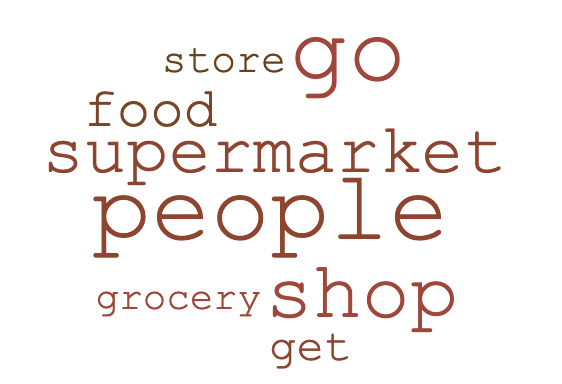
\includegraphics[width=1.4in]{images/topic1.png}
%\caption{fig1}
\end{minipage}%
}%
\subfigure[topic 2]{
\begin{minipage}[t]{0.3\linewidth}
\centering
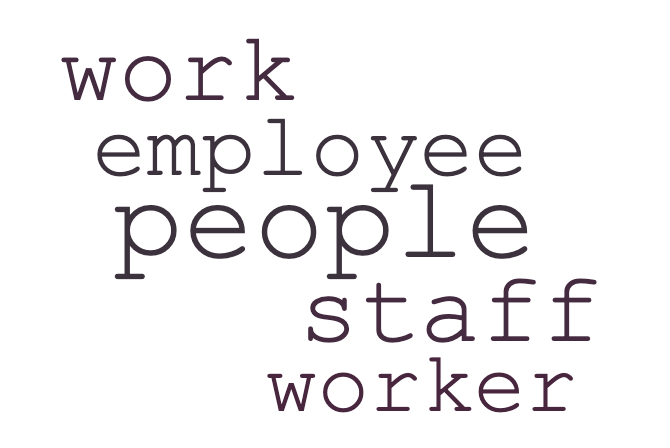
\includegraphics[width=1.4in]{images/topic2.png}
%\caption{fig2}
\end{minipage}%
}%

\subfigure[topic 4]{
\begin{minipage}[t]{0.3\linewidth}
\centering
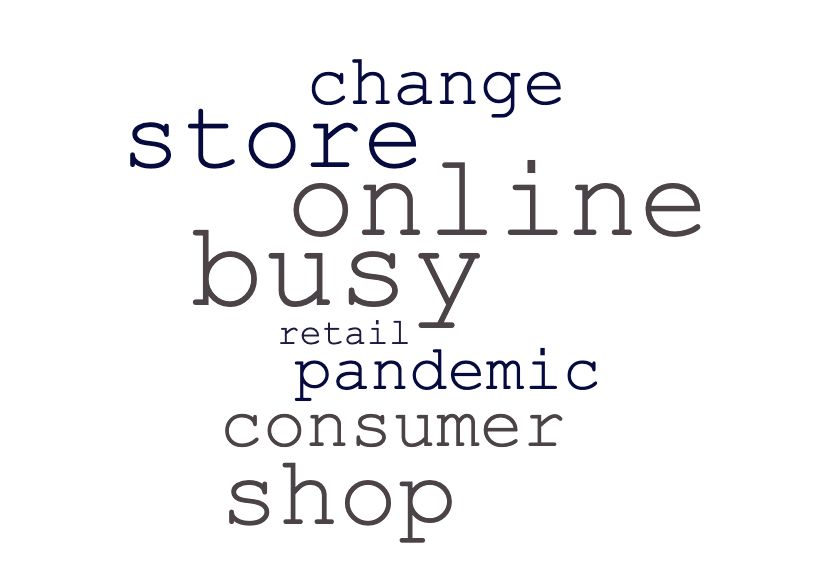
\includegraphics[width=1.4in]{images/topic4.png}
%\caption{fig2}
\end{minipage}
}%
\subfigure[topic 8]{
\begin{minipage}[t]{0.3\linewidth}
\centering
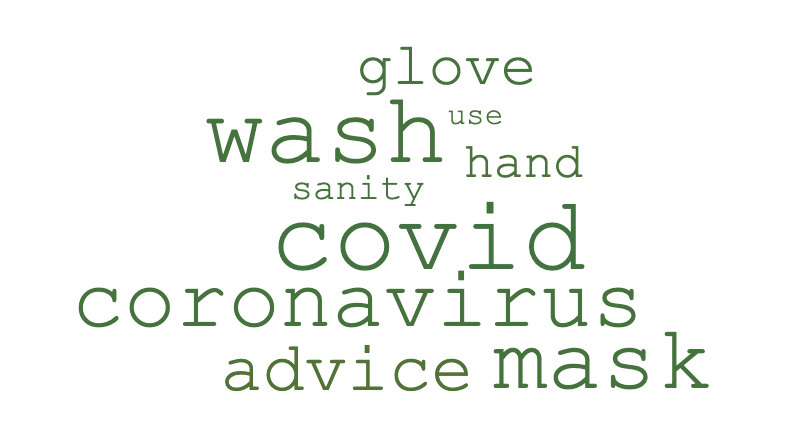
\includegraphics[width=1.4in]{images/topic8.png}
%\caption{fig2}
\end{minipage}
}%
\centering
\caption{Examples of Word Cloud}
\label{fig:9}
\end{figure}

As for the second application, we trained TTM with a relatively various dataset and use the trained model to infer the input COVID-19 related dataset to find the topic distribution in a period of time. A google news dataset contains over ten thousand documents with over 150 topics, but after cursory observation, it is found that the topics generated by the google news dataset are not highly relevant to the content of our Twitter dataset. Therefore, we still used the SearchSnippets dataset but preprocessing by the same techniques of the Twitter dataset. \ref{table_6} shows the trained result with the processed SearchSnippets dataset. Most of the generated topics are interpretable and it can be clearly to distinguish that the topics are related to science and subject (topic 1 \& 8), computer (topic 2), polity (topic 4), music and movie (topic 3 \& 5), sports (topic 6) and health (topic 7).

\begin{table}[htbp]
\centering
\begin{tabular}{|c|c|}
\hline
Topic ID & Top words\\
\hline
1 & \tabincell{l}{research edu science busy inform \\market program com journal}\\
\hline
2 & \tabincell{l}{software computer web program system \\internet memory intel com network}\\
\hline
3 & \tabincell{l}{music com car art engineer \\electric online buy home}\\
\hline
4 & \tabincell{l}{polity culture wikipedia system party \\government encyclopedia inform wiki}\\
\hline
5 & \tabincell{l}{movie com film video news \\fashion award art photo}\\
\hline
6 & \tabincell{l}{sport news game football com \\soccer ticket team match}\\
\hline
7 & \tabincell{l}{health inform cancer medical gov \\disease news research drug}\\
\hline
8 & \tabincell{l}{amazon book theory wikipedia encyclopedia \\com physics mathematical theoretical}\\
\hline
\end{tabular}
\caption{Training Result}
\label{table_6}
\end{table}

We randomly selected 500 Tweets samples each day to estimate the whole topics distribution in that day to discover the variation of topics in the second half of March (early stage of the outbreak). Since the lack of data between Mar. $27^{th}$ and Apr. $1^{st}$, we divided the data in those days into two parts (three days for one part), and selected 500 Tweets in each part. Additionally, with the purpose to find the topic variation during the pandemic, we use a line chart instead of a bar chart in the design, which is more clear to discover the evolution of topics. The line chart for variation of the topics in the second half of March is shown as figure \ref{fig:12}, where the x-axis denotes the date, the y-axis denotes the number of Tweets assigned to each topic (in the 500 samples Tweets) and different colors denote different topics. 

\begin{figure}[H]
    \centering
    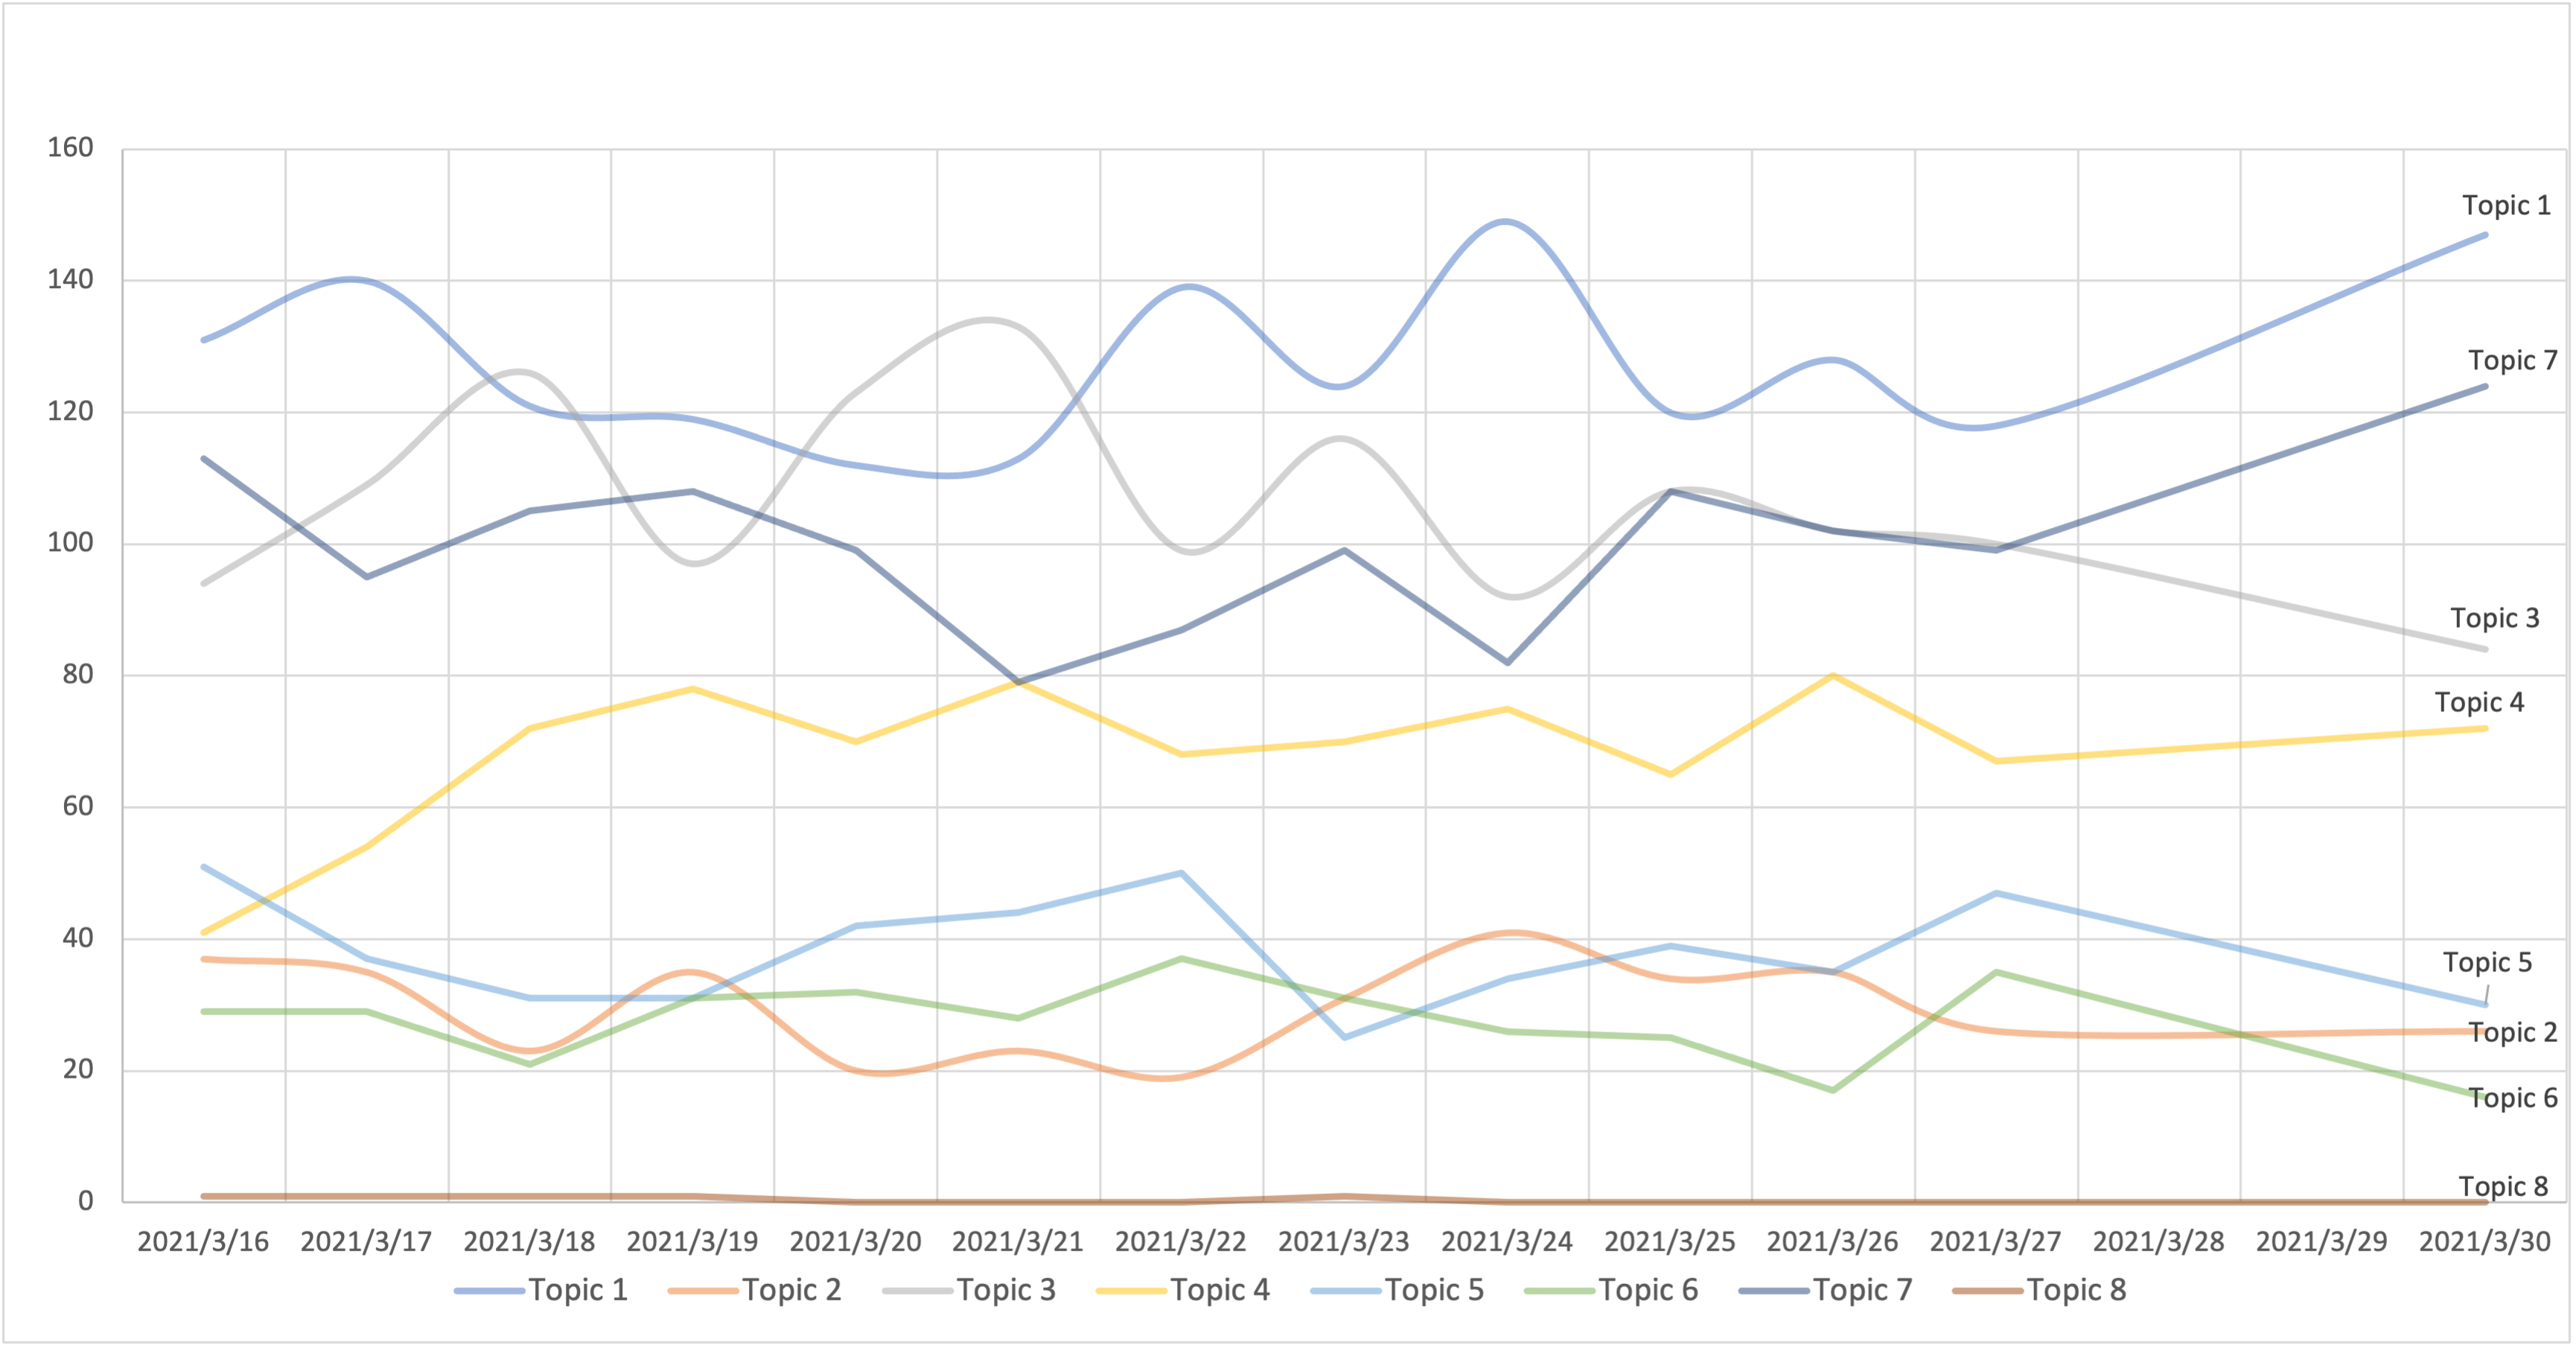
\includegraphics[scale=0.6]{images/topic_distribution.png}
    \caption{Variation of Topic Distribution}
    \label{fig:12}
\end{figure}

The above result shows that the distribution of most topics in the second half of March tends to stabilize. Topic 1 and topic 7 are mentioned frequently and have continuing upward trend. Topic 3, which seems to be related to online shopping and music, is also popular but might reduce in April. The topic about politics is rarely discussed at the beginning, but increases significantly afterwards. While other topics such as the topics related to movies and sports are not mentioned too much during the pandemic. 

There is a certain degree of rationality for the above analysis of the change of topics in half month at the early stage of the outbreak. For example, it is clear that the discussions on the topics related to health and government have increased with the severity of the epidemic, which accords with the reality. And we can infer from the curve of topic 7 that after around one week from the outbreak, people start to pay more attention to the epidemic disease and their health. But because of the limited topics in the training dataset, there might be a lot of Tweets cannot be assigned to the right topic (since their topic may not be included in the training set), which will influence the result of the topic distribution. Moreover, the period of a half month is still quite short and cannot get more information for the analysis of public response. Therefore, the next stage of the project is to find a suitable training set with more topics and apply it on discovering the variation of topic distribution in a longer period of time during the pandemic to capture the public response to COVID-19.